\chapter{Residual Stress and FWHM Prediction}
\label{chap: reg}

Because of the efficiency of ultrasonic testings in terms of inspection area and cost, we explore the potential of using ultrasonic testings to measure quantities of interest, residual stress and full width at half maximum (FWHM), which are originally obtained from XRD analysis. In this chapter, we present regression models for predicting the residual stress and the FWHM of XRD peaks in fatigue damaged samples based on the ultrasonic measurements. 

\section{Problem formulation}
Following the same manner in Section \ref{sec: rul prob formulation}, we first translate the prediction tasks into ML regression problems based on the available dataset.

\subsection{Dataset}
The dataset for predicting residual stress and FWHM is composed of the XRD results and ultrasonic measurements. To obtain the residual stress and FWHM, the XRD analysis was performed on a subset of samples, containing 8 specimens and 3 measurement locations for each specimen, in the RUL dataset. Table \ref{table: rs dataset} and \ref{table: fwhm dataset} are the summary of the residual stress and FWHM dataset, respectively. It is observed that specimen 7's relatively low FWHM values could indicate that there are microcrack initiations, and the discussion about cracks in specimen 7 is presented in Section \ref{sec: reg discussion}.

\begin{table}[tb]
    \centering
    \caption{Summary of the residual stress prediction dataset}
    \label{table: rs dataset}
    \begin{tabularx}{\textwidth}{
      >{\centering\arraybackslash}X|
      >{\centering\arraybackslash}X|
      >{\centering\arraybackslash}X|
      >{\centering\arraybackslash}X
    }
    \hline
    & \multicolumn{3}{c}{Residual Stress (MPa)}\\
    \hline
      Specimen ID & Location 1 & Location 2 & Location 3\\
      \hline
      2 & -61.7 & -75.6 & -80.2 \\
      4 & -59.9 & -69.6 & -76.6 \\
      6 & -60.3 & -75.3 & -79.6 \\
      7 & -50.8 & -59.6 & -66.2 \\
      8 & -57.3 & -65.5 & -79.7 \\
      10 & -43.3 & -47.0 & -50.8 \\
      12 & -38.8 & -43.2 & -50.0 \\
      14 & -79 & -76.7 & -85.7 \\
      \hline
    \end{tabularx}

    \footnotesize{The negative sign indicates the compressive residual stresses.}
\end{table}


\begin{table}[tb]
    \centering
    \caption{Summary of the FWHM prediction dataset}
    \label{table: fwhm dataset}
    \begin{tabularx}{\textwidth}{
      >{\centering\arraybackslash}X|
      >{\centering\arraybackslash}X|
      >{\centering\arraybackslash}X|
      >{\centering\arraybackslash}X
    }
    \hline
    & \multicolumn{3}{c}{FWHM ($^{\circ}$)}\\
    \hline
      Specimen ID & Location 1 & Location 2 & Location 3\\
      \hline
      2 & 0.354 & 0.353 & 0.355 \\
      4 & 0.350 & 0.354 & 0.353 \\
      6 & 0.358 & 0.359 & 0.363 \\
      7 & 0.307 & 0.320 & 0.321 \\
      8 & 0.357 & 0.355 & 0.358 \\
      10 & 0.356 & 0.358 & 0.360 \\
      12 & 0.354 & 0.353 & 0.355 \\
      14 & 0.338 & 0.340 & 0.346 \\
      \hline

    \end{tabularx}
\end{table}

\subsection{Target variables}
Residual stress and FWHM are the target variables in this chapter. Residual stress is known to influence fatigue behaviors including crack initiation and propagation. FWHM is also an indicator for evaluating crack propagation. As a result, accurately predicting residual stress and FWHM based on ultrasonic measurements is beneficial to assist fatigue level estimation. Here, the problem is formulated as two regression tasks separately:
\begin{enumerate*}[label=(\alph*)]
    \item a univariate regression with residual stress as the target variable, and
    \item a univariate regression with FWHM as the target variable.
\end{enumerate*}


\section{Residual stress prediction}
\label{sec: rs prediction}
A regression model, RFECV-SVM\textsubscript{RS}, for predicting residual stress based on ultrasonic signals is developed by following the procedure in Chapter \ref{chap: model}. Besides, the RFECV-SVM\textsubscript{RS} model is compared with other approaches such as Lasso regression, linear regression with top 5 features from Lasso regression, and random forest. Root mean squared error (RMSE) and mean absolute percentage error (MAPE) are used to assess the model performance with LOGOCV results, as shown in Table \ref{table: summary rs model}. In this task, the RFECV-SVM\textsubscript{RS} model performs the best with the MAPE equal 4.73\%. Figure \ref{fig: rs prediction} illustrates the RFECV-SVM\textsubscript{RS} model prediction by showing the actual and predicted residual stresses, in which a perfect model should follow the black line. It is observed that in most groups, at least one prediction among three repeated measurements (three predictions for the same actual residual stress in one sample group) is close to the ideal prediction, and the MAPEs for each group are mostly below 10\%.

\begin{table}[tb]
    \centering
    \caption{Summary of regression models for residual stress estimation and model performance}
    \label{table: summary rs model}
    \begin{tabularx}{\textwidth}{
      >{\centering\arraybackslash}X
      >{\centering\arraybackslash}X
      >{\centering\arraybackslash\hsize=0.8\hsize}X
      >{\centering\arraybackslash\hsize=0.8\hsize}X
    }
    \toprule
    \multirow{2}{*}{Method}  & \multirow{2}{*}{\parbox{\linewidth}{\centering No. Selected \\ Features}} & \multicolumn{2}{c}{LOGOCV Test} \\
    \cmidrule(lr){3-4}
    & & RMSE (MPa) & MAPE (\%) \\
    \midrule
    %
    Lasso regression & 37 & 5.90 & 8.71 \\
    Linear regression & 5 & 4.92 & 7.54 \\
    Random forest & 283 & 7.74 & 12.85 \\
    RFECV-SVM & 29 & 3.24 & 4.73 \\
    \bottomrule
    \end{tabularx}
\end{table}

\begin{figure}[tb]
  \centering
  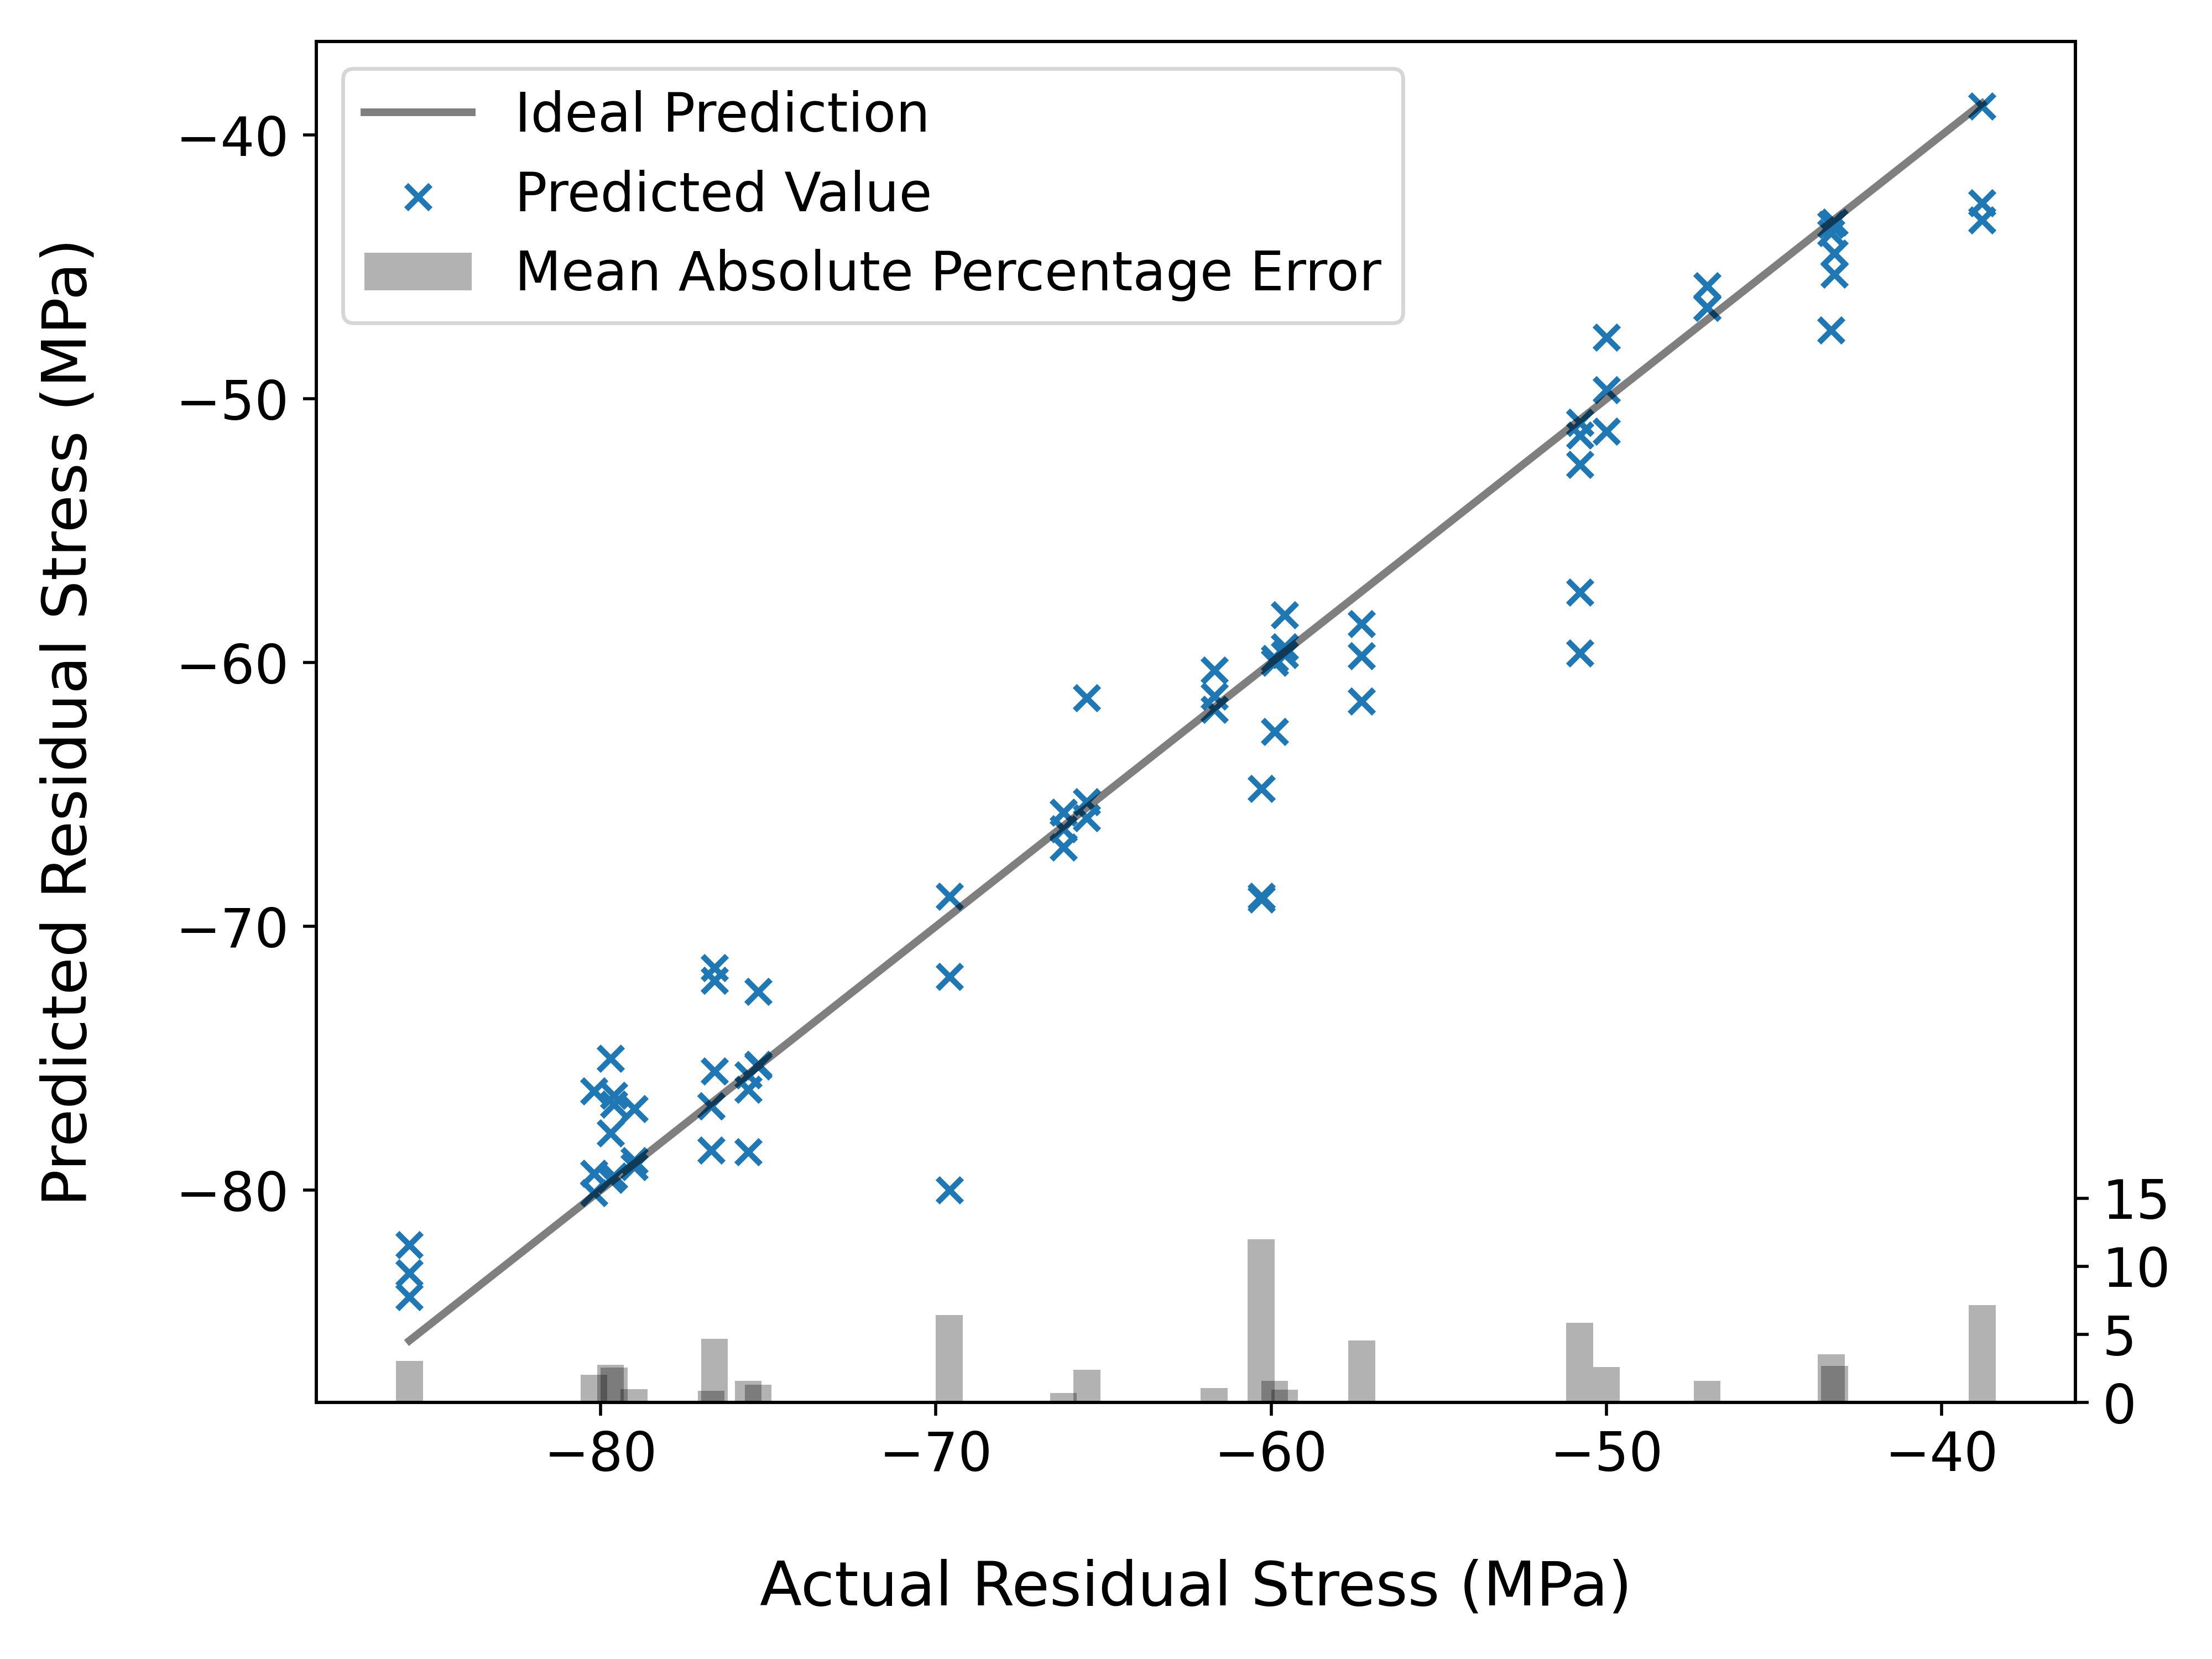
\includegraphics[width=0.8\linewidth]{fig/residual_stress_predict_vs_true.png}
  \caption{Scatter plot of actual vs predicted residual stress by RFECV-SVM}
  \label{fig: rs prediction}
\end{figure}

\section{FWHM prediction}
Similarly, an FWHM prediction model, RFECV-SVM\textsubscript{FWHM}, is built based on the procedure in Chapter \ref{chap: model} and is evaluated with the same metrics in Section \ref{sec: rs prediction}. Table \ref{table: summary fwhm model} is the comparison of the RFECV-SVM\textsubscript{FWHM} with other regression methods. It is worth mentioning that the linear regression model with the top 5 features selected from Lasso regression achieves a 1.89\% MAPE, performing slightly better than the RFECV-SVM\textsubscript{FWHM}. Figure \ref{fig: fwhm prediction lr} and \ref{fig: fwhm prediction svm} illustrate the predictions of the linear regression model and the RFECV-SVM\textsubscript{FWHM}, respectively. For the RFECV-SVM\textsubscript{FWHM}, one can observe that the predictions of the small FWHM values from specimen 7 significantly deviate from the ideal predictions; nevertheless, the linear regression model is able to make close predictions. As mentioned earlier, we surmise that specimen 7 had developed cracks and the difference in the model performance led us to have a further investigation about specimen 7 in Section \ref{sec: reg discussion}. Before performing further analysis, by excluding specimen 7, we can conclude that both models achieve a good performance in predicting FWHM with errors less than 2\%.

\begin{table}[tb]
  \centering
  \caption{Summary of regression models for FWHM prediction and model performance}
  \label{table: summary fwhm model}
  \begin{tabularx}{\textwidth}{
    >{\centering\arraybackslash}X
    >{\centering\arraybackslash}X
    >{\centering\arraybackslash\hsize=0.8\hsize}X
    >{\centering\arraybackslash\hsize=0.8\hsize}X
  }
  \toprule
  \multirow{2}{*}{Method}  & \multirow{2}{*}{\parbox{\linewidth}{\centering No. Selected \\ Features}} & \multicolumn{2}{c}{LOGOCV Test} \\
  \cmidrule(lr){3-4}
  & & RMSE (\textcolor{red}{unit}) & MAPE (\%) \\
  \midrule
  %
  Lasso regression & 20 & 0.0081 & 2.40 \\
  Linear regression & 5 & 0.0056 & 1.62 \\
  Random forest & 283 & 0.0099 & 2.81 \\
  RFECV-SVM & 7 & 0.0063 & 1.89 \\
  \bottomrule
  \end{tabularx}
\end{table}

\begin{figure}[tb]
  \centering
  \begin{subfigure}[t]{\linewidth}
    \centering
    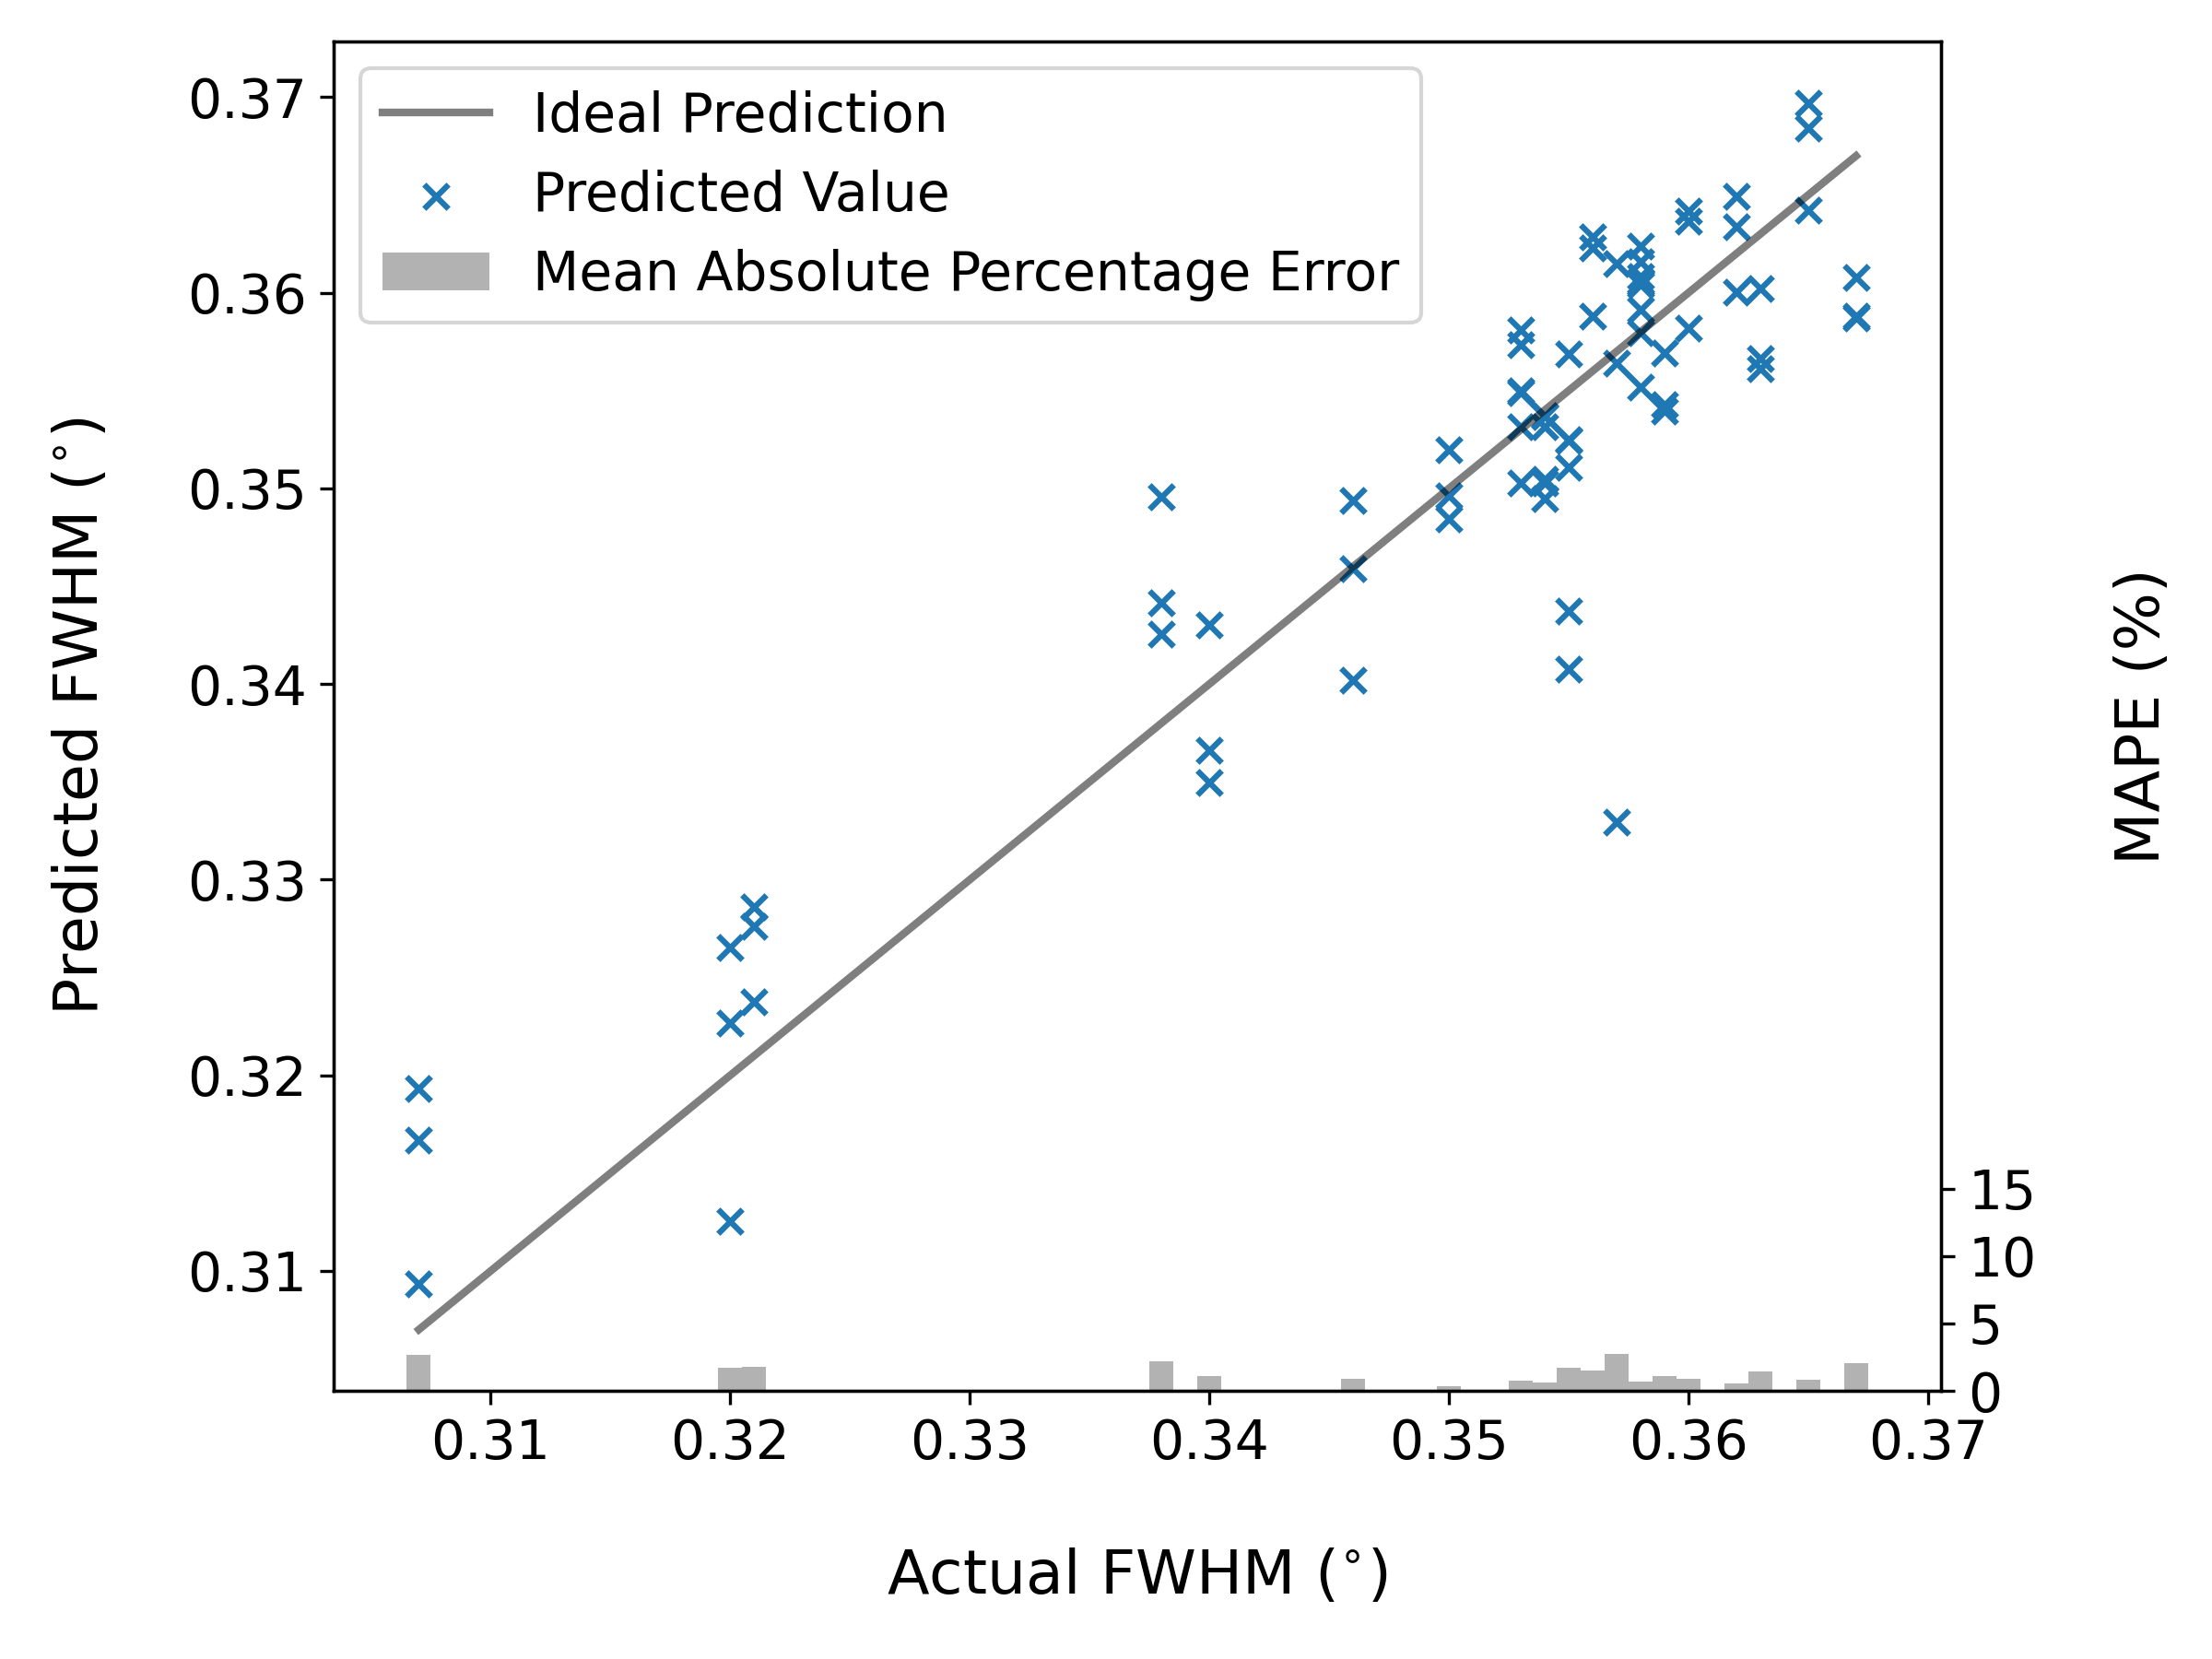
\includegraphics[width=0.8\linewidth]{fig/fwhm_predict_vs_true_lr.png}
    \caption{Linear regression}
    \label{fig: fwhm prediction lr}
  \end{subfigure}
  \begin{subfigure}[t]{\linewidth}
    \centering
    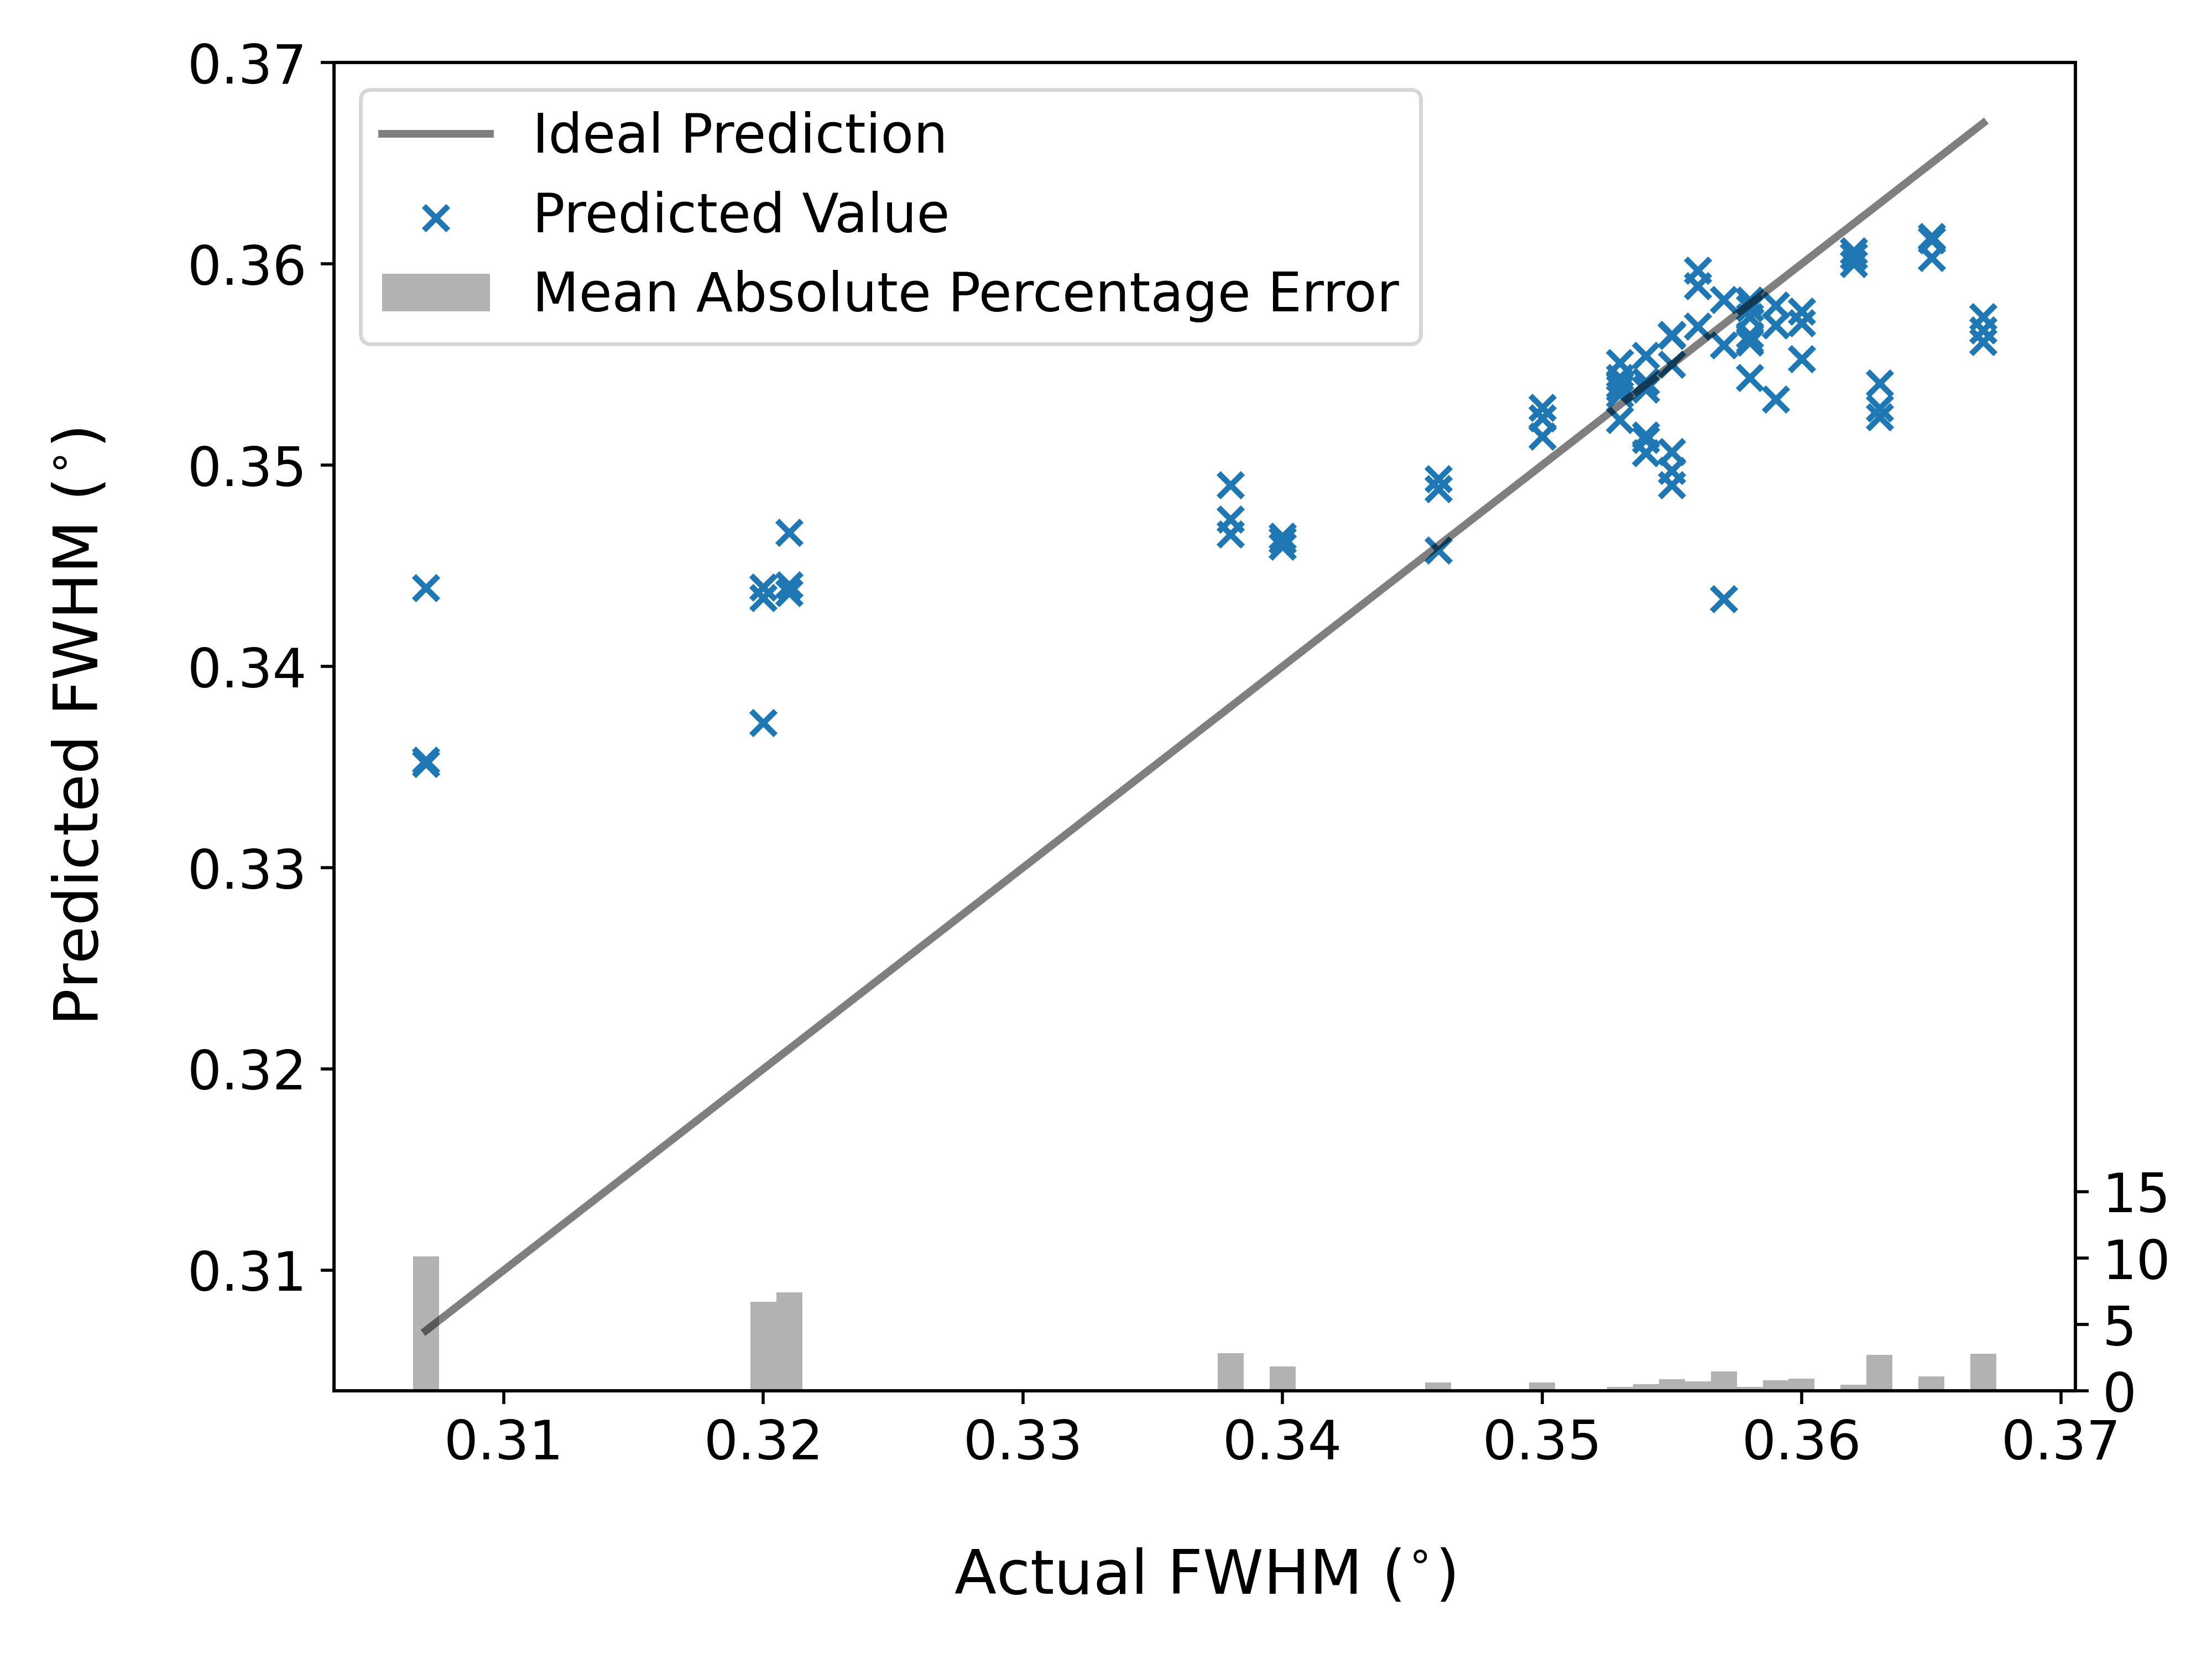
\includegraphics[width=0.8\linewidth]{fig/fwhm_predict_vs_true_svm.png}
    \caption{RFECV-SVM}
    \label{fig: fwhm prediction svm}
  \end{subfigure}

  \caption{Scatter plot of actual vs predicted FWHM}
  \label{fig: fwhm prediction}
\end{figure}

\section{Discussion}
\label{sec: reg discussion}
In this section, since we conjecture that specimen 7 had developed cracks based on the relatively small FWHM values measured from XRD analysis, the potential of using our ultrasonic technology to detect cracks is discussed.

\subsection{Crack detection through LU and NLU measurements}
To investigate whether our ultrasonic technology can detect cracks or not, we first assume specimen 7 is cracked and the differences in ultrasonic signals between specimen 7 and specimen 8 were resulted from the existence of cracks since specimen 7 and 8 were under the same experimental setting. Secondly, independent t-test is performed to test if the mean of a feature is significantly different between two groups, specimen 7 (15 measurements from location 3a to 3) and specimen 8 (15 measurements from location 3a to 3). Finally, Figure \ref{fig: crack detection feat dist} displays several specimen 7's and specimen 8's probability density plots of the selected features. The distributions are not identical between specimen 7 and 8, indicating that these features are possible to distinguish cracked samples from normal samples; however, given that we only have two specimens in this test and there exist other factors causing the differences in measurement signals, further research on crack detection through our ultrasonic technology is required.

\begin{figure}[tb]
  \begin{subfigure}[t]{0.49\linewidth}
    \centering
    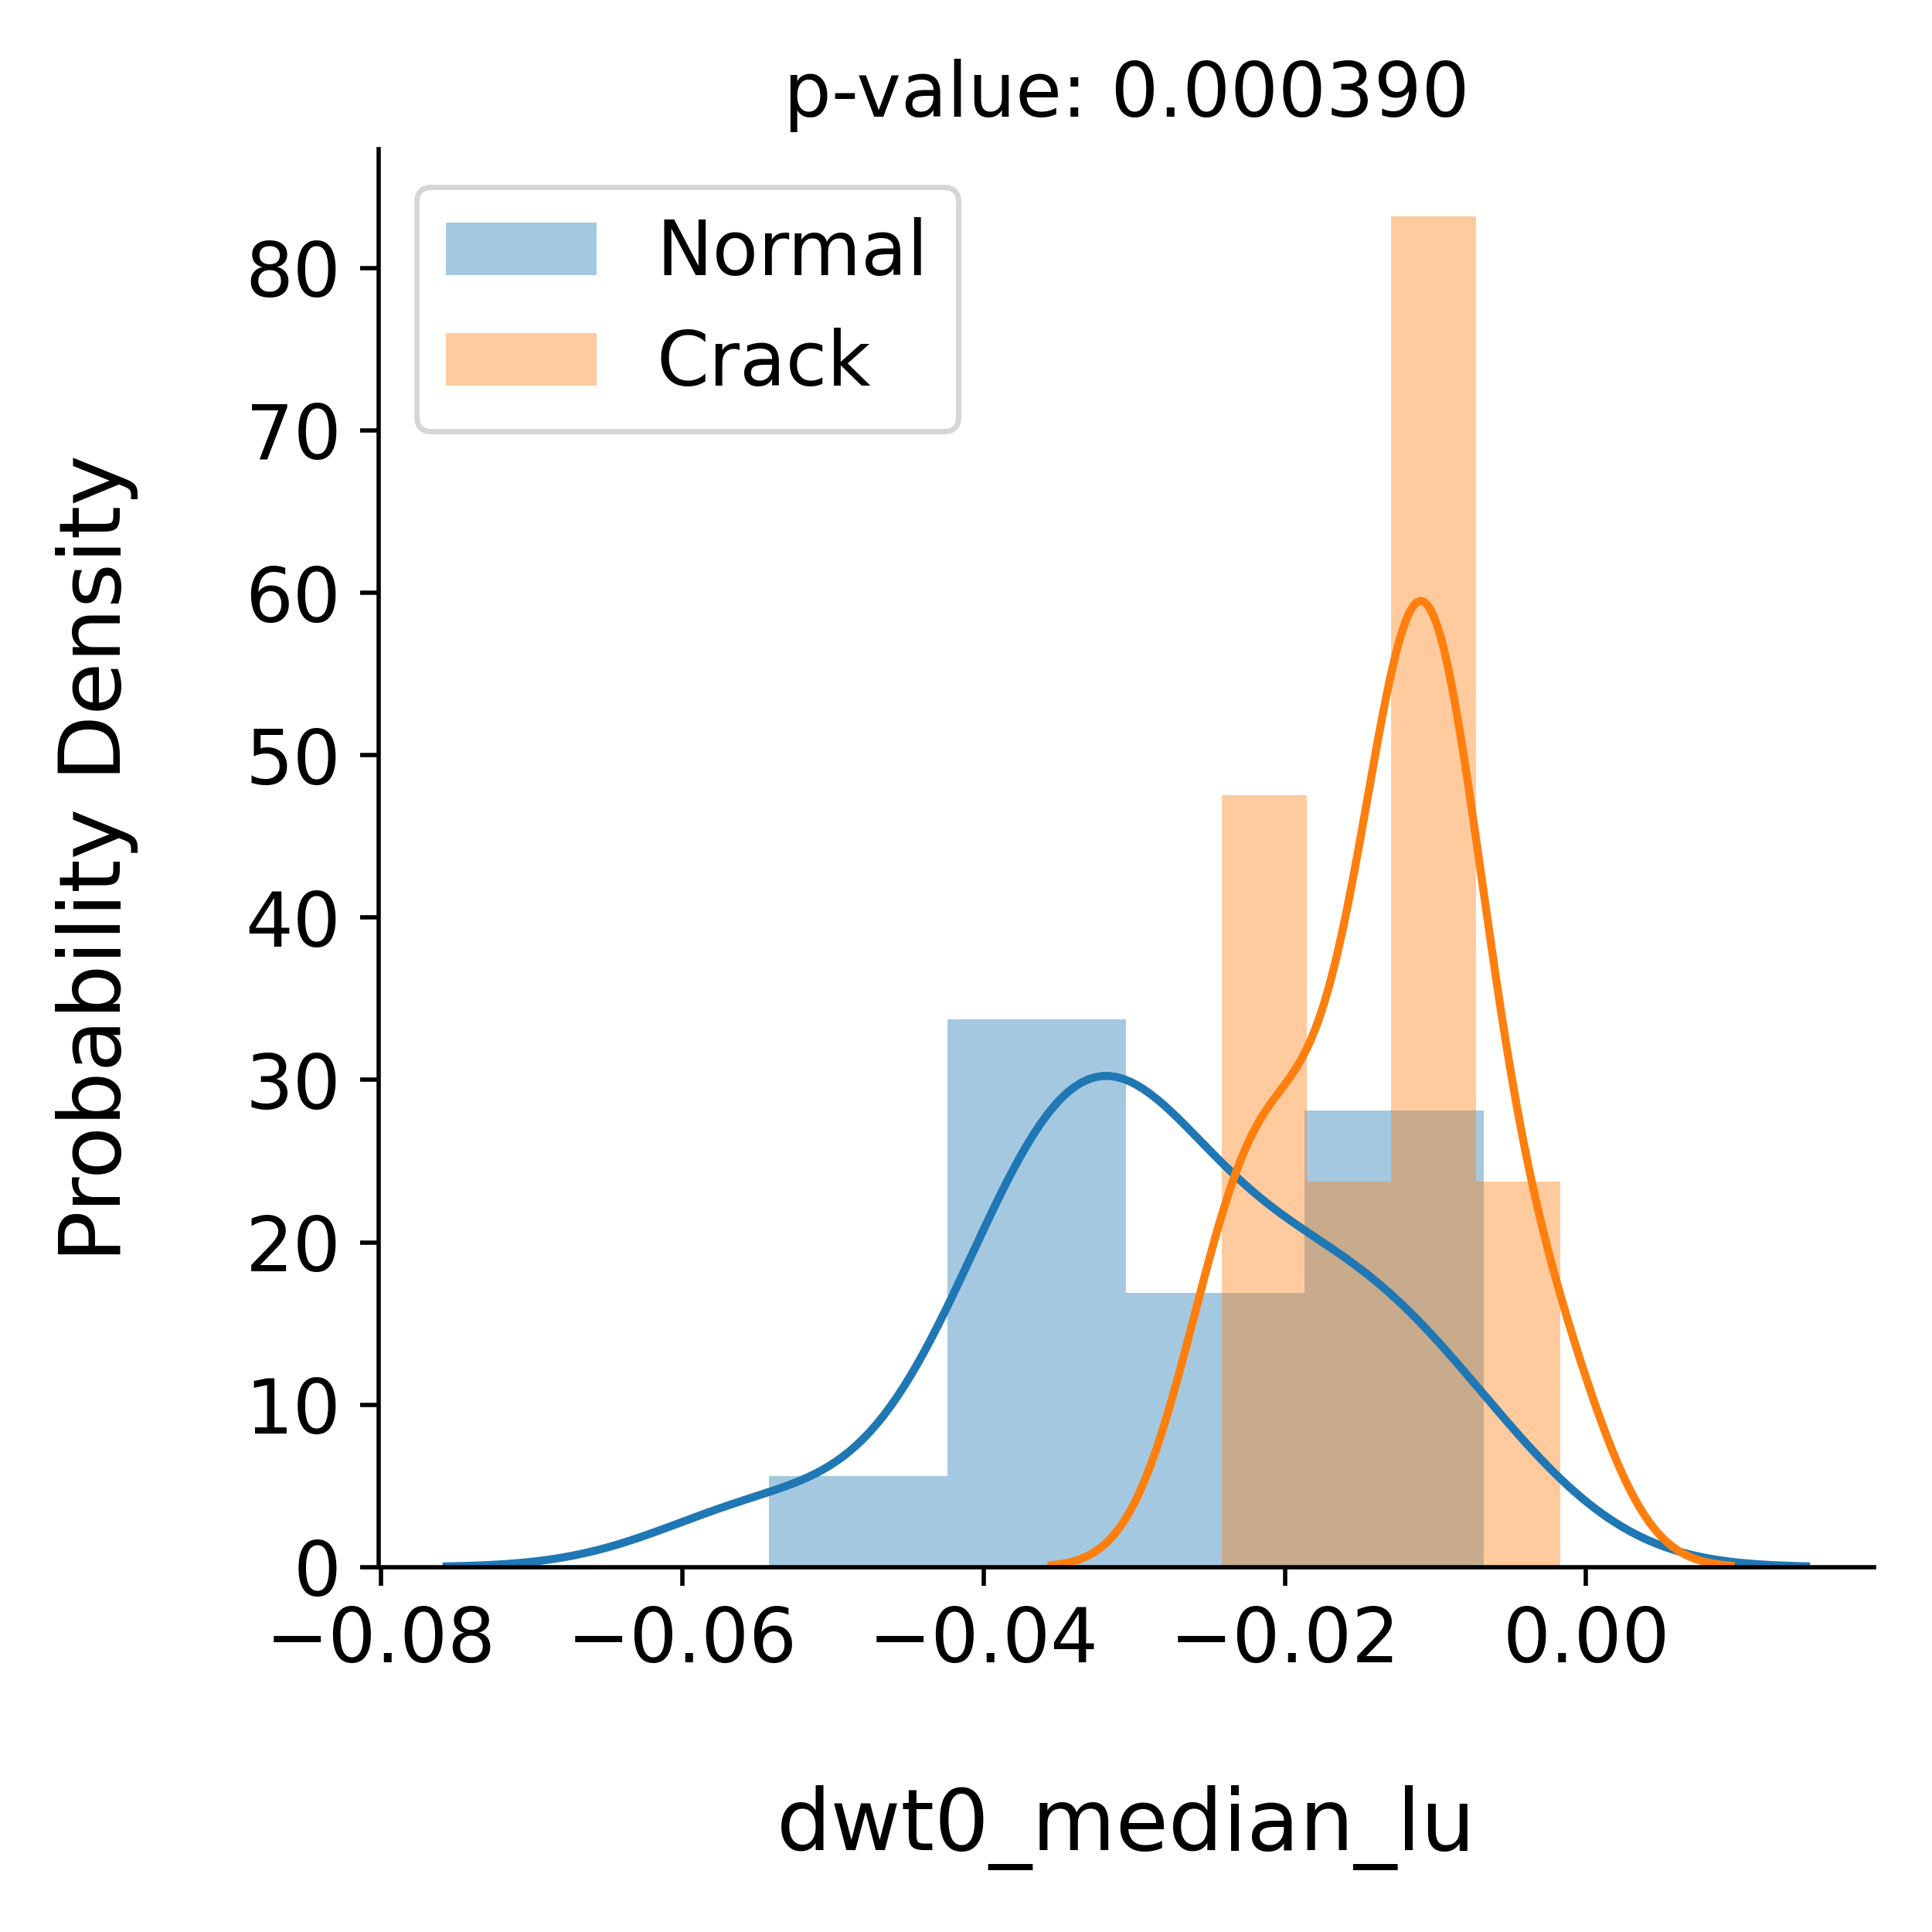
\includegraphics[width=0.8\textwidth]{fig/crack_detection_dwt0_median_lu.png}
    \caption{Median of level 0 DWT coefficient of LU signal}
  \end{subfigure}
  \begin{subfigure}[t]{0.49\linewidth}
    \centering
    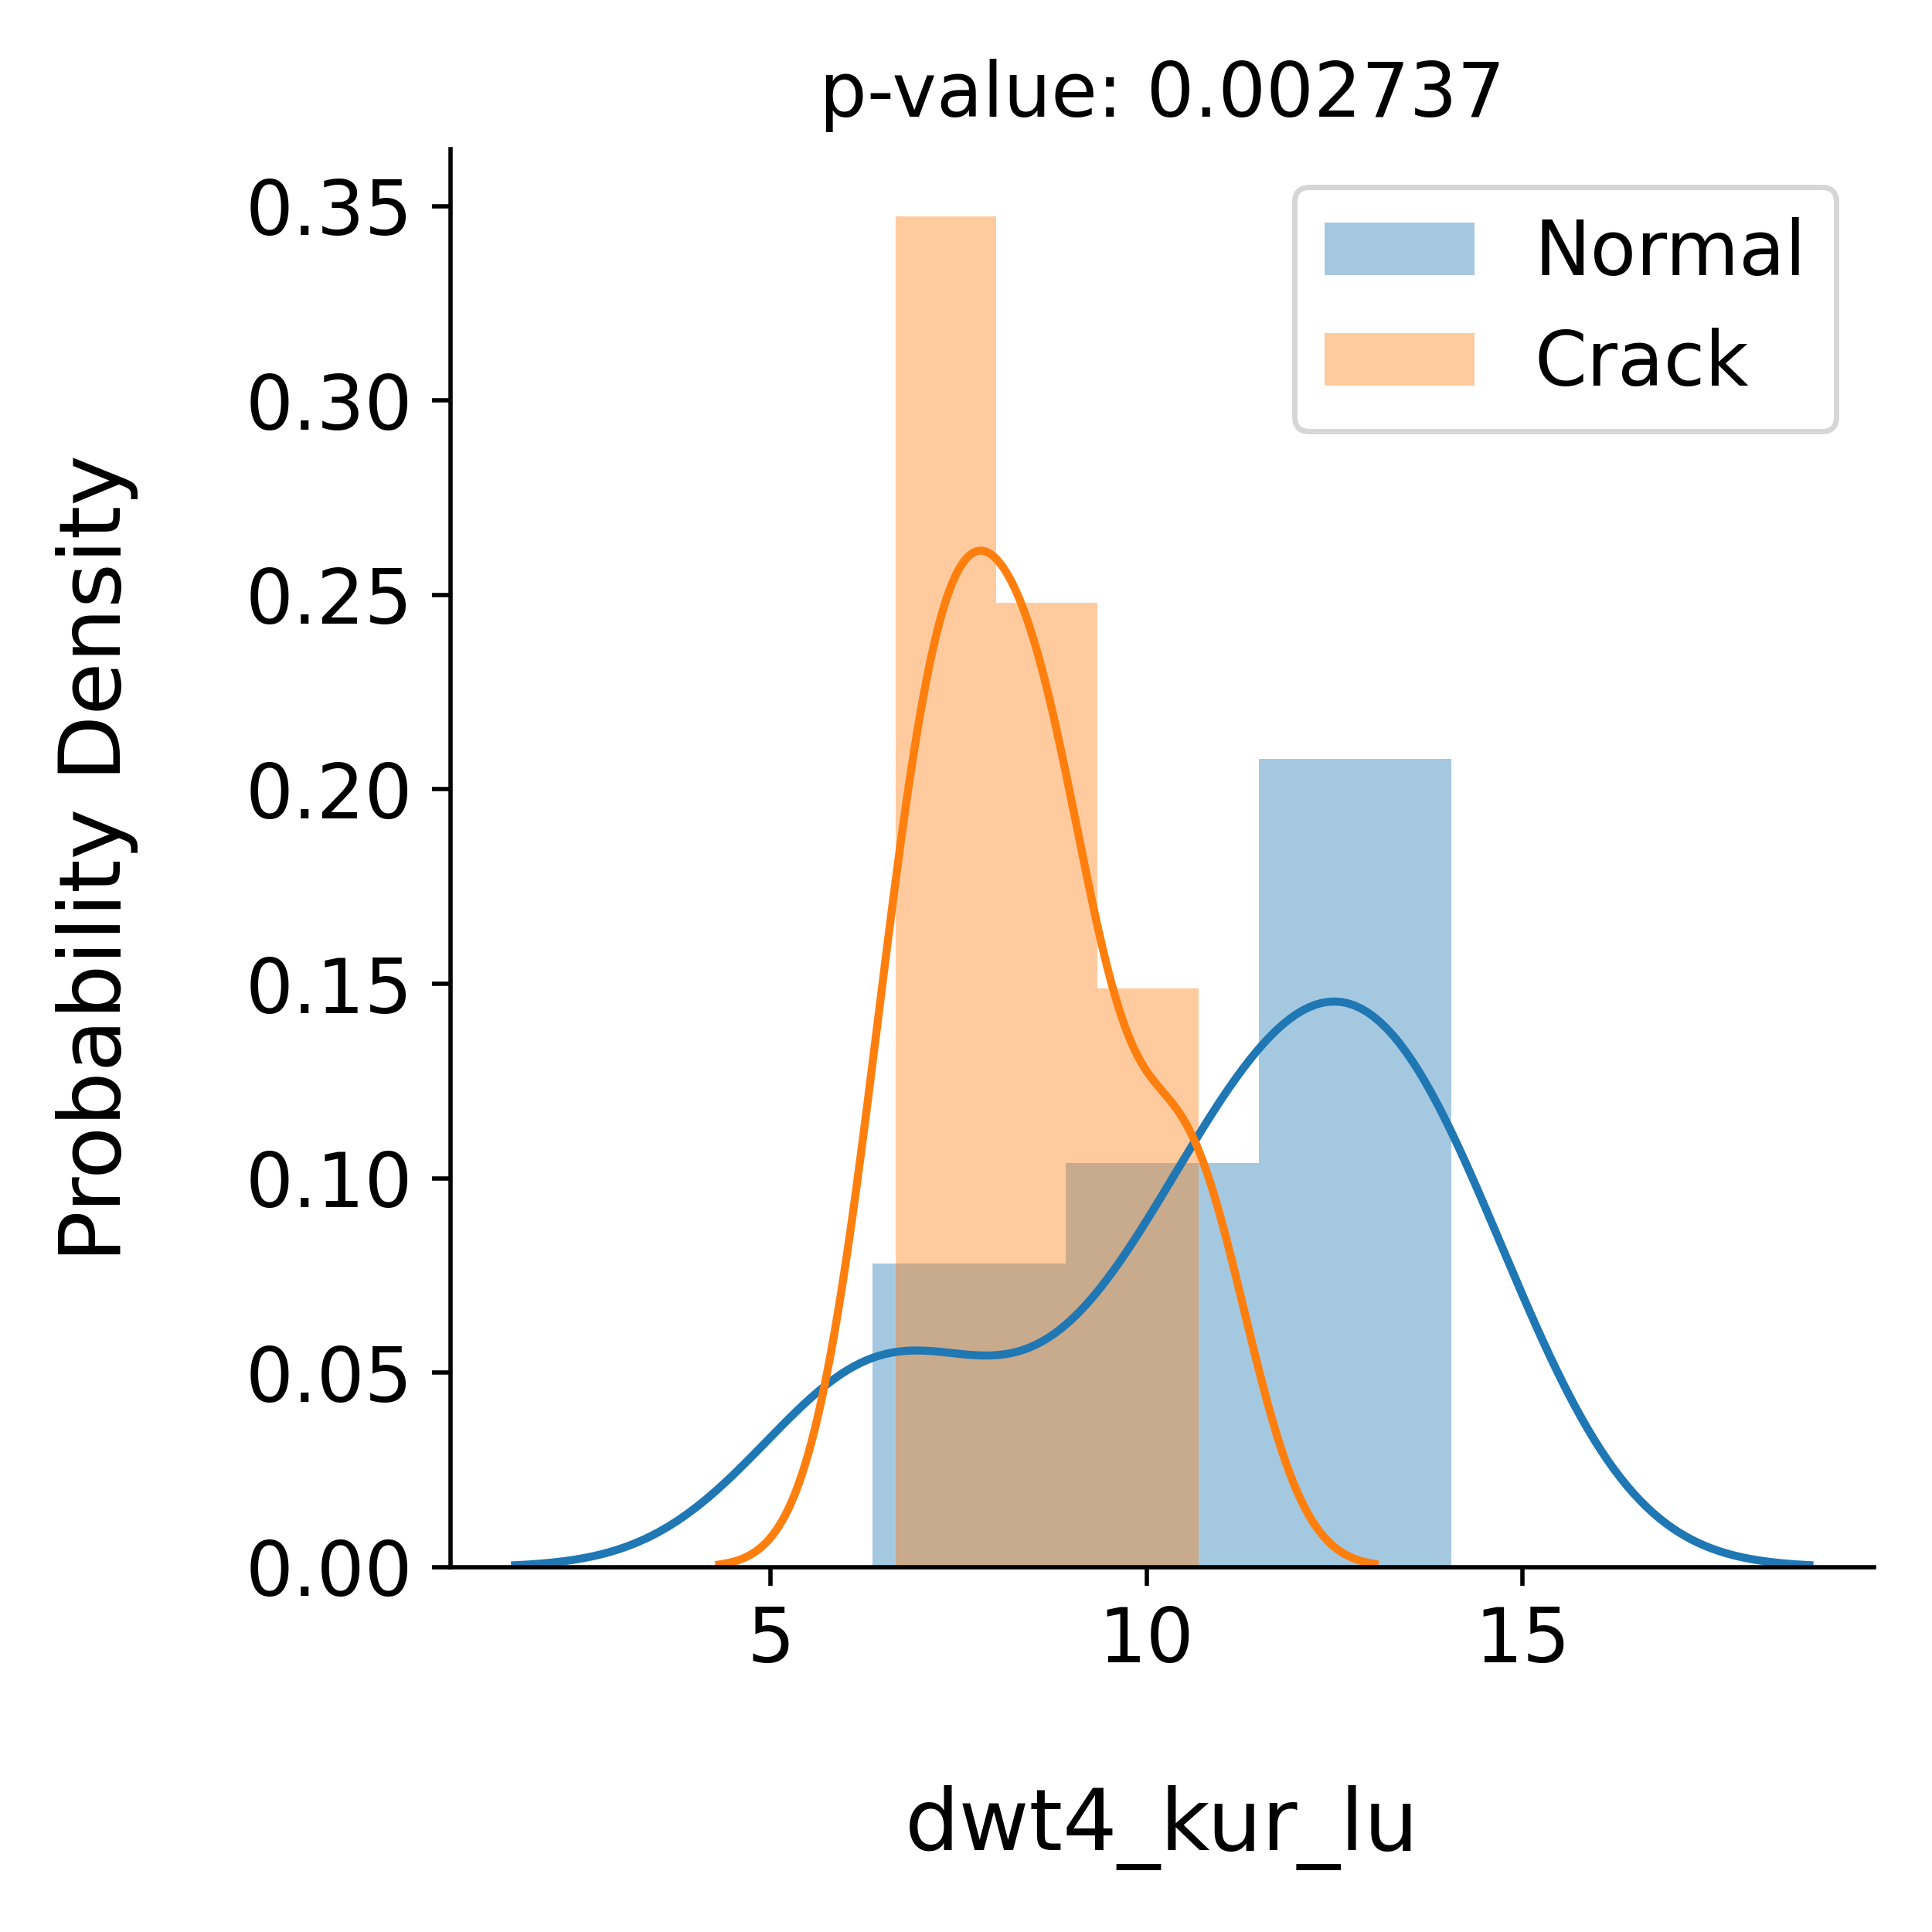
\includegraphics[width=0.8\textwidth]{fig/crack_detection_dwt4_kur_lu.png}
    \caption{Kurtosis of level 4 DWT coefficient of LU signal}
  \end{subfigure}
  \begin{subfigure}[t]{0.49\linewidth}
    \centering
    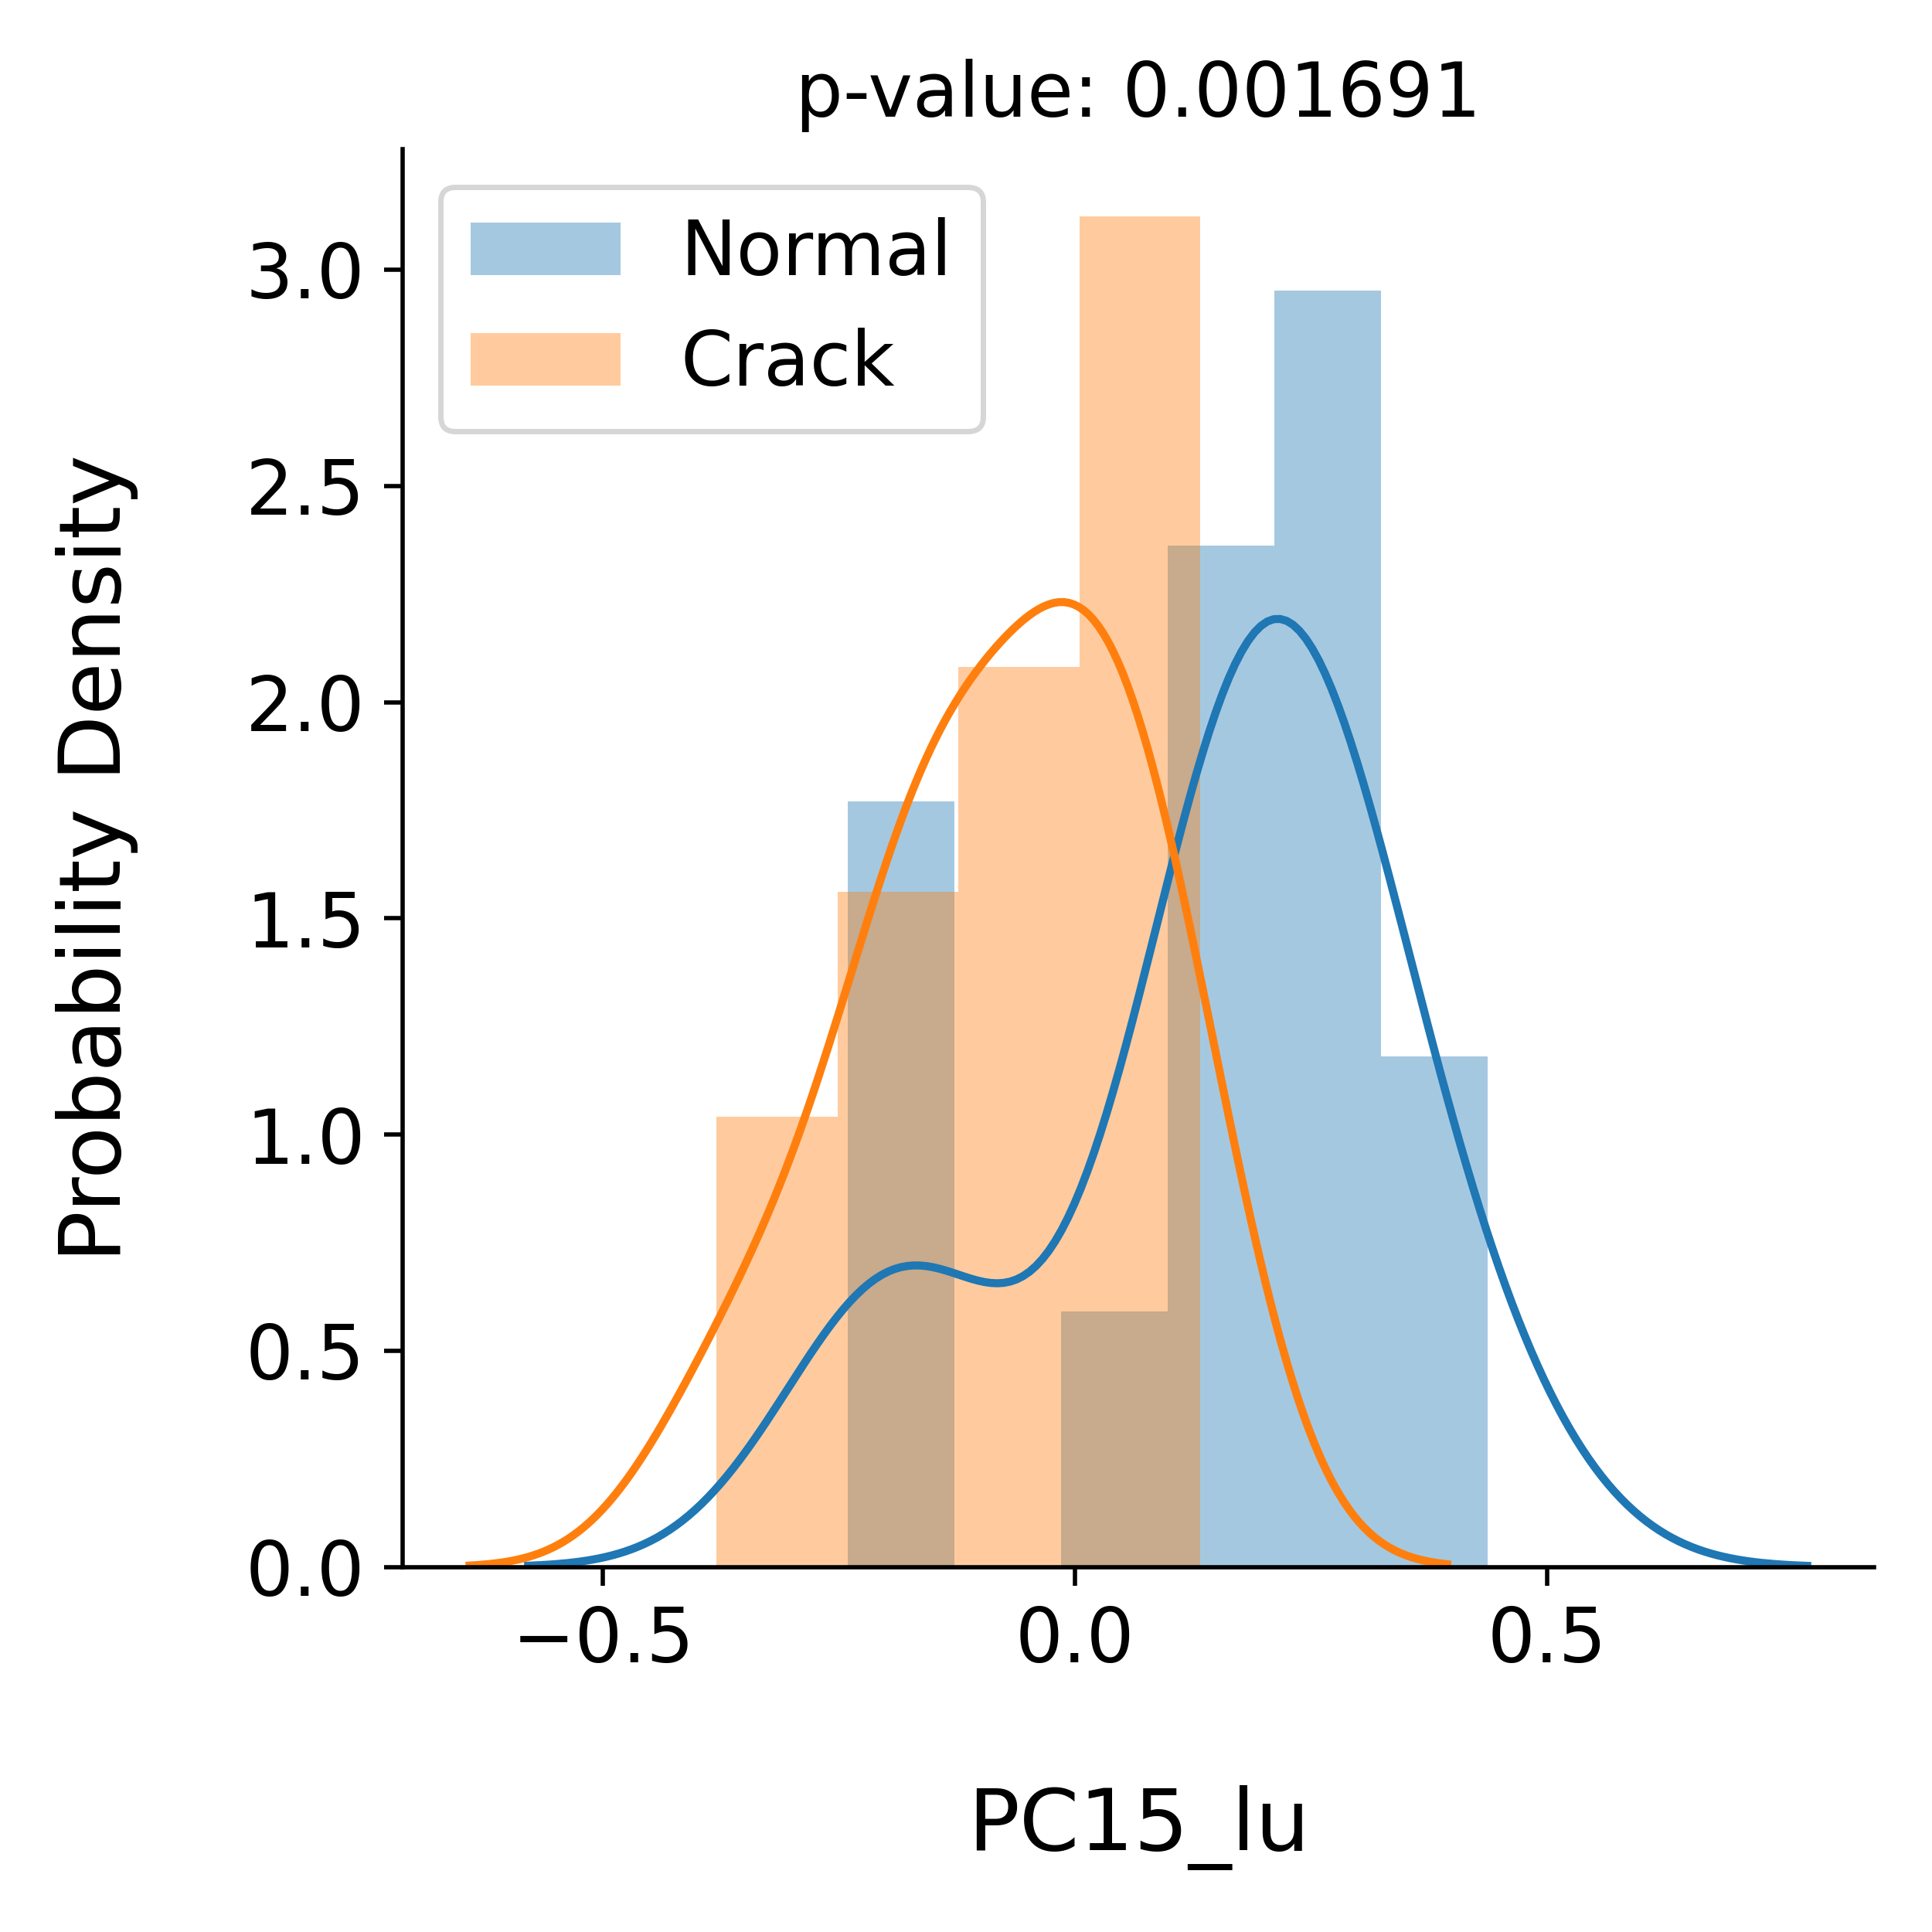
\includegraphics[width=0.8\textwidth]{fig/crack_detection_PC15_lu.png}
    \caption{Principal component 15 of LU signal}
  \end{subfigure}
  \begin{subfigure}[t]{0.49\linewidth}
    \centering
    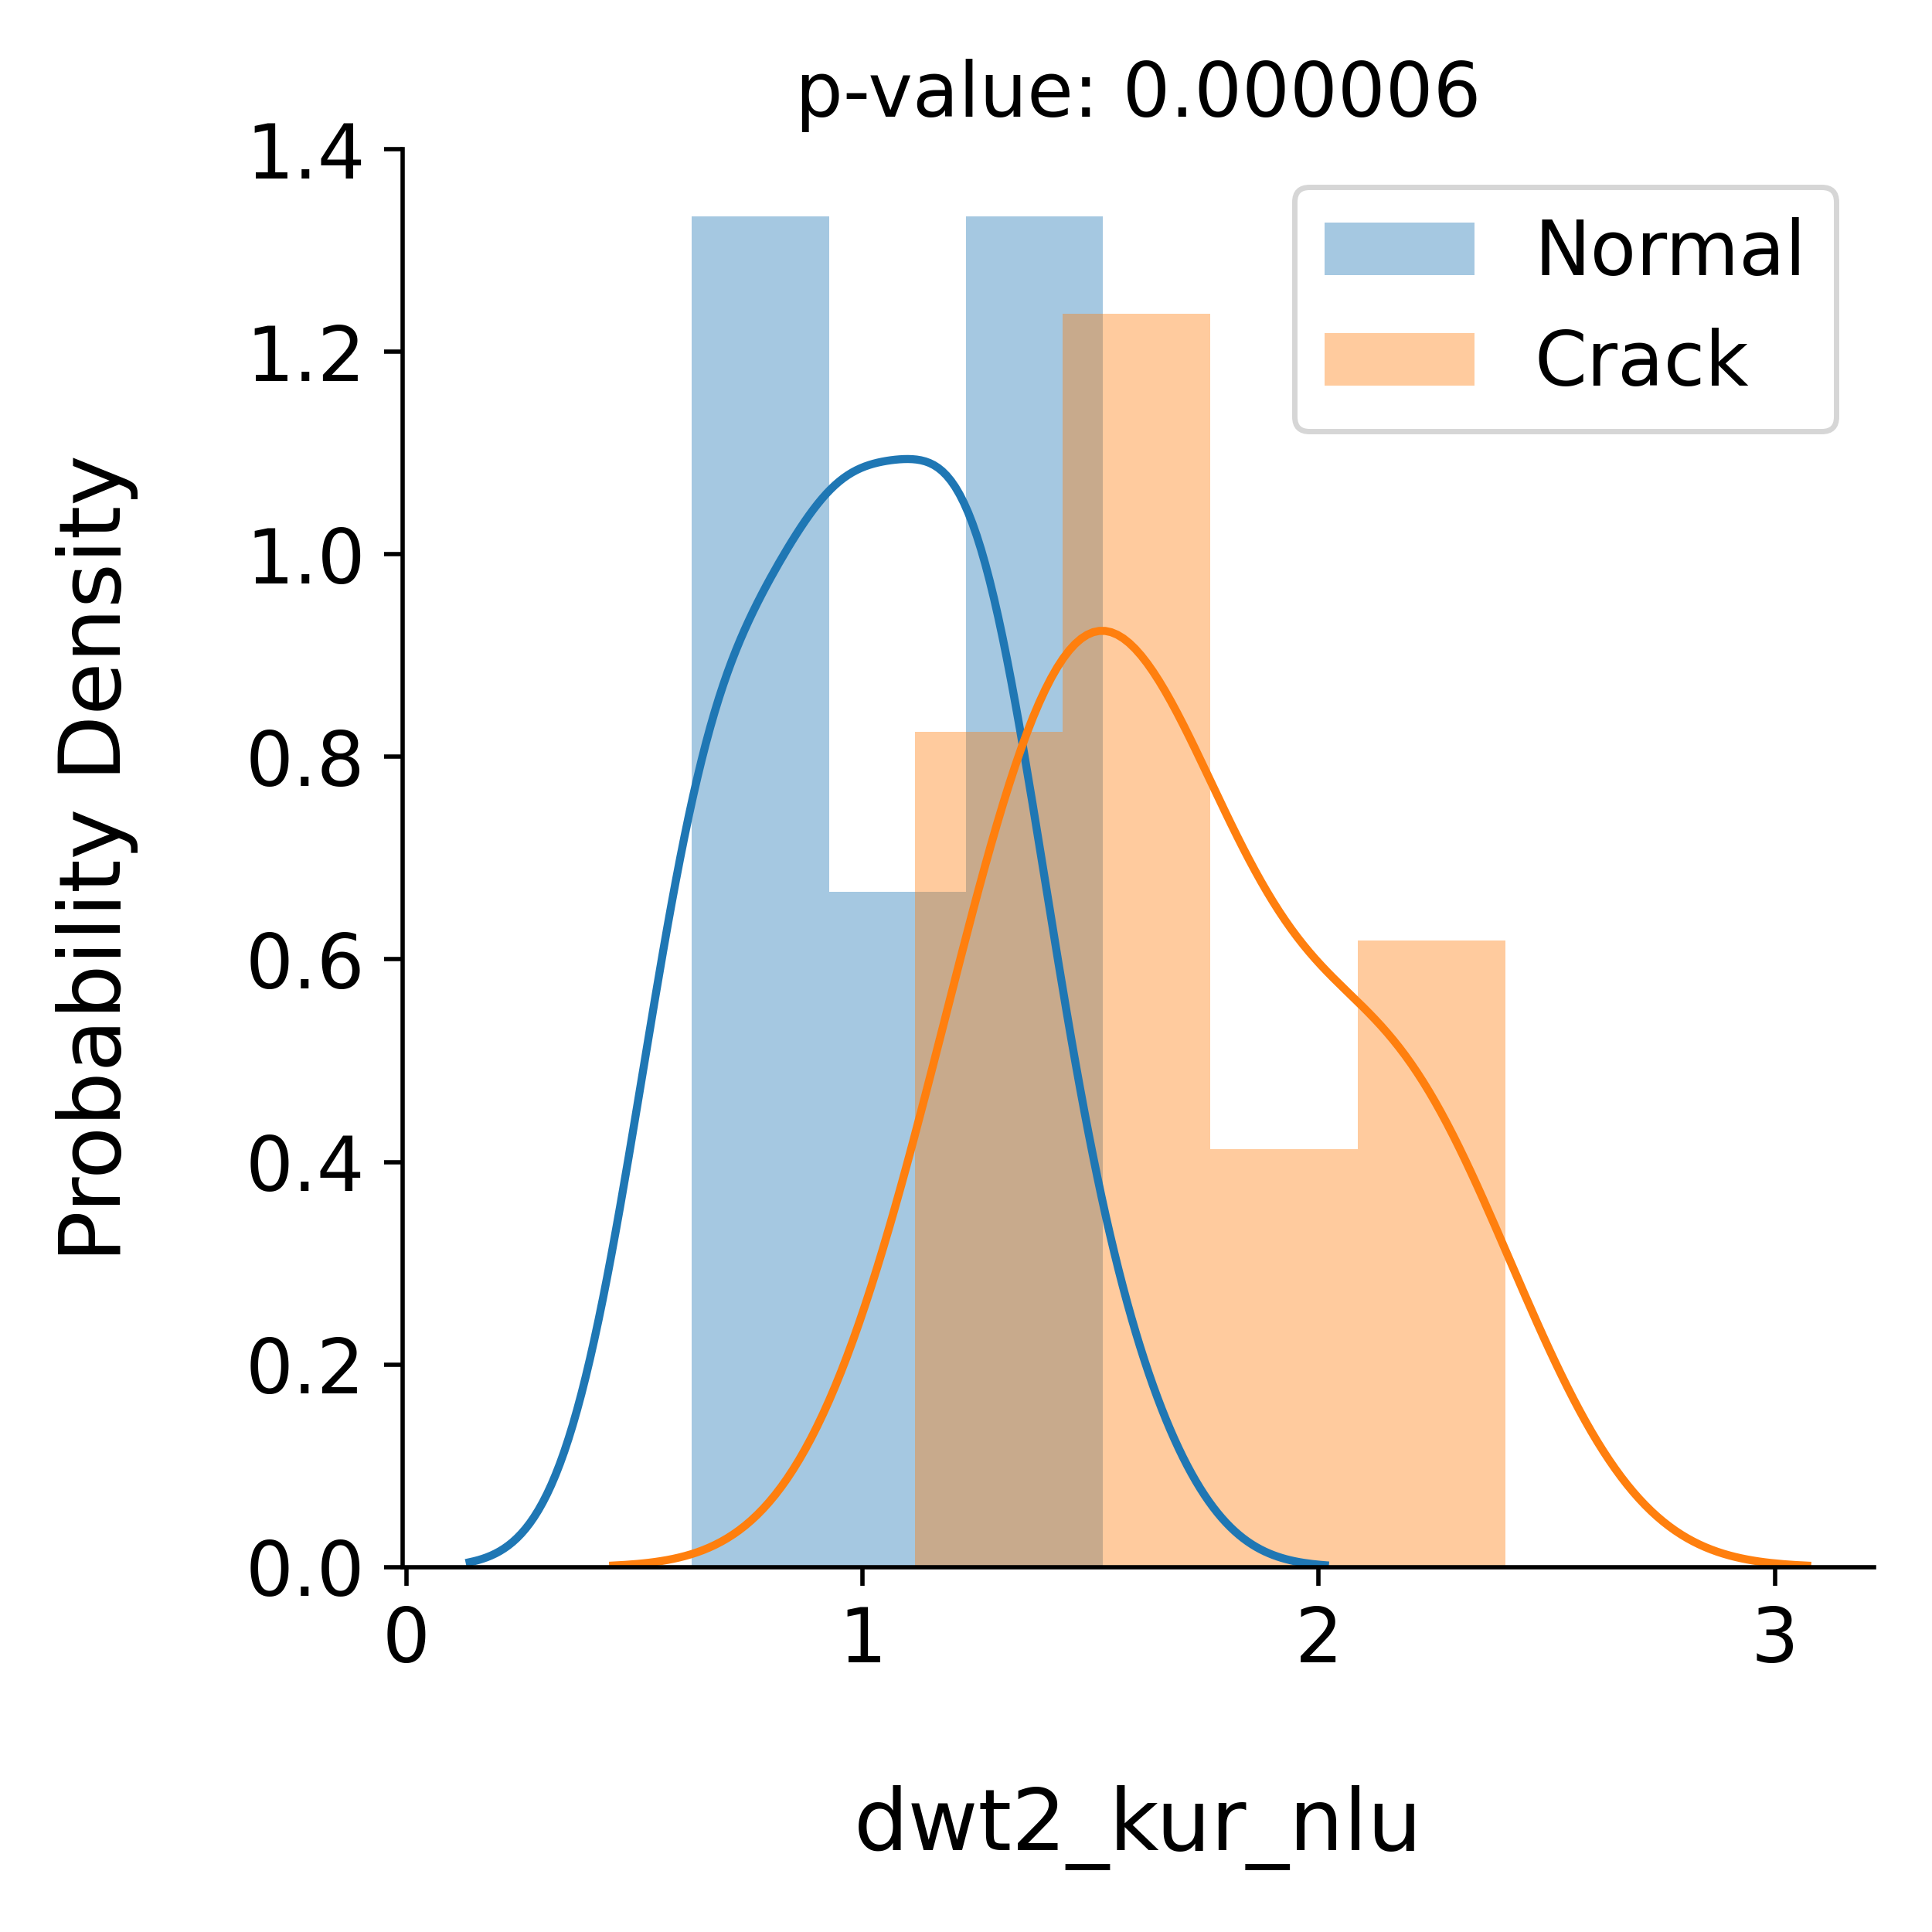
\includegraphics[width=0.8\textwidth]{fig/crack_detection_dwt2_kur_nlu.png}
    \caption{Kurtosis of level 2 DWT coefficient of NLU signal}
  \end{subfigure}
  \begin{subfigure}[t]{0.49\linewidth}
    \centering
    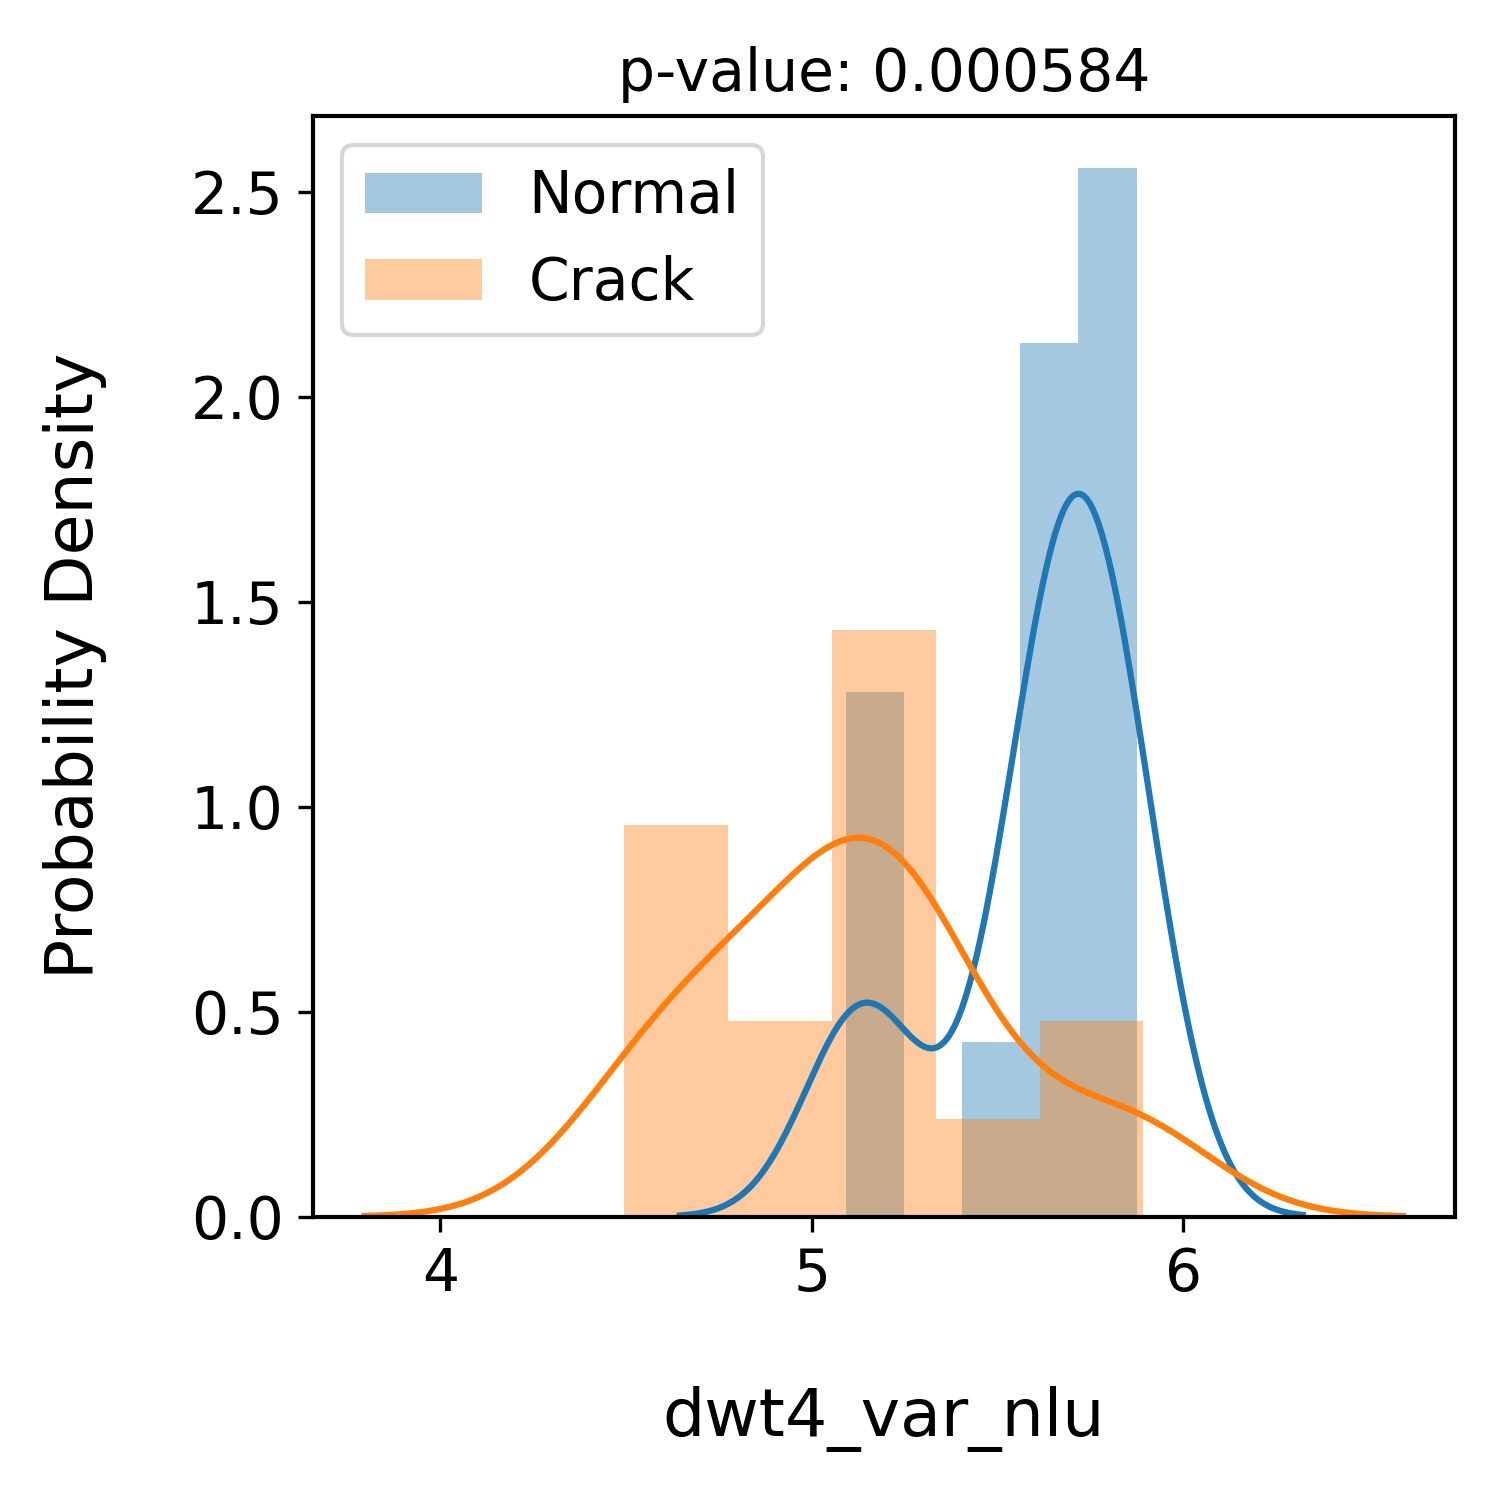
\includegraphics[width=0.8\textwidth]{fig/crack_detection_dwt4_var_nlu.png}
    \caption{Variance of level 4 DWT coefficient of NLU signal}
  \end{subfigure}
  \begin{subfigure}[t]{0.49\linewidth}
    \centering
    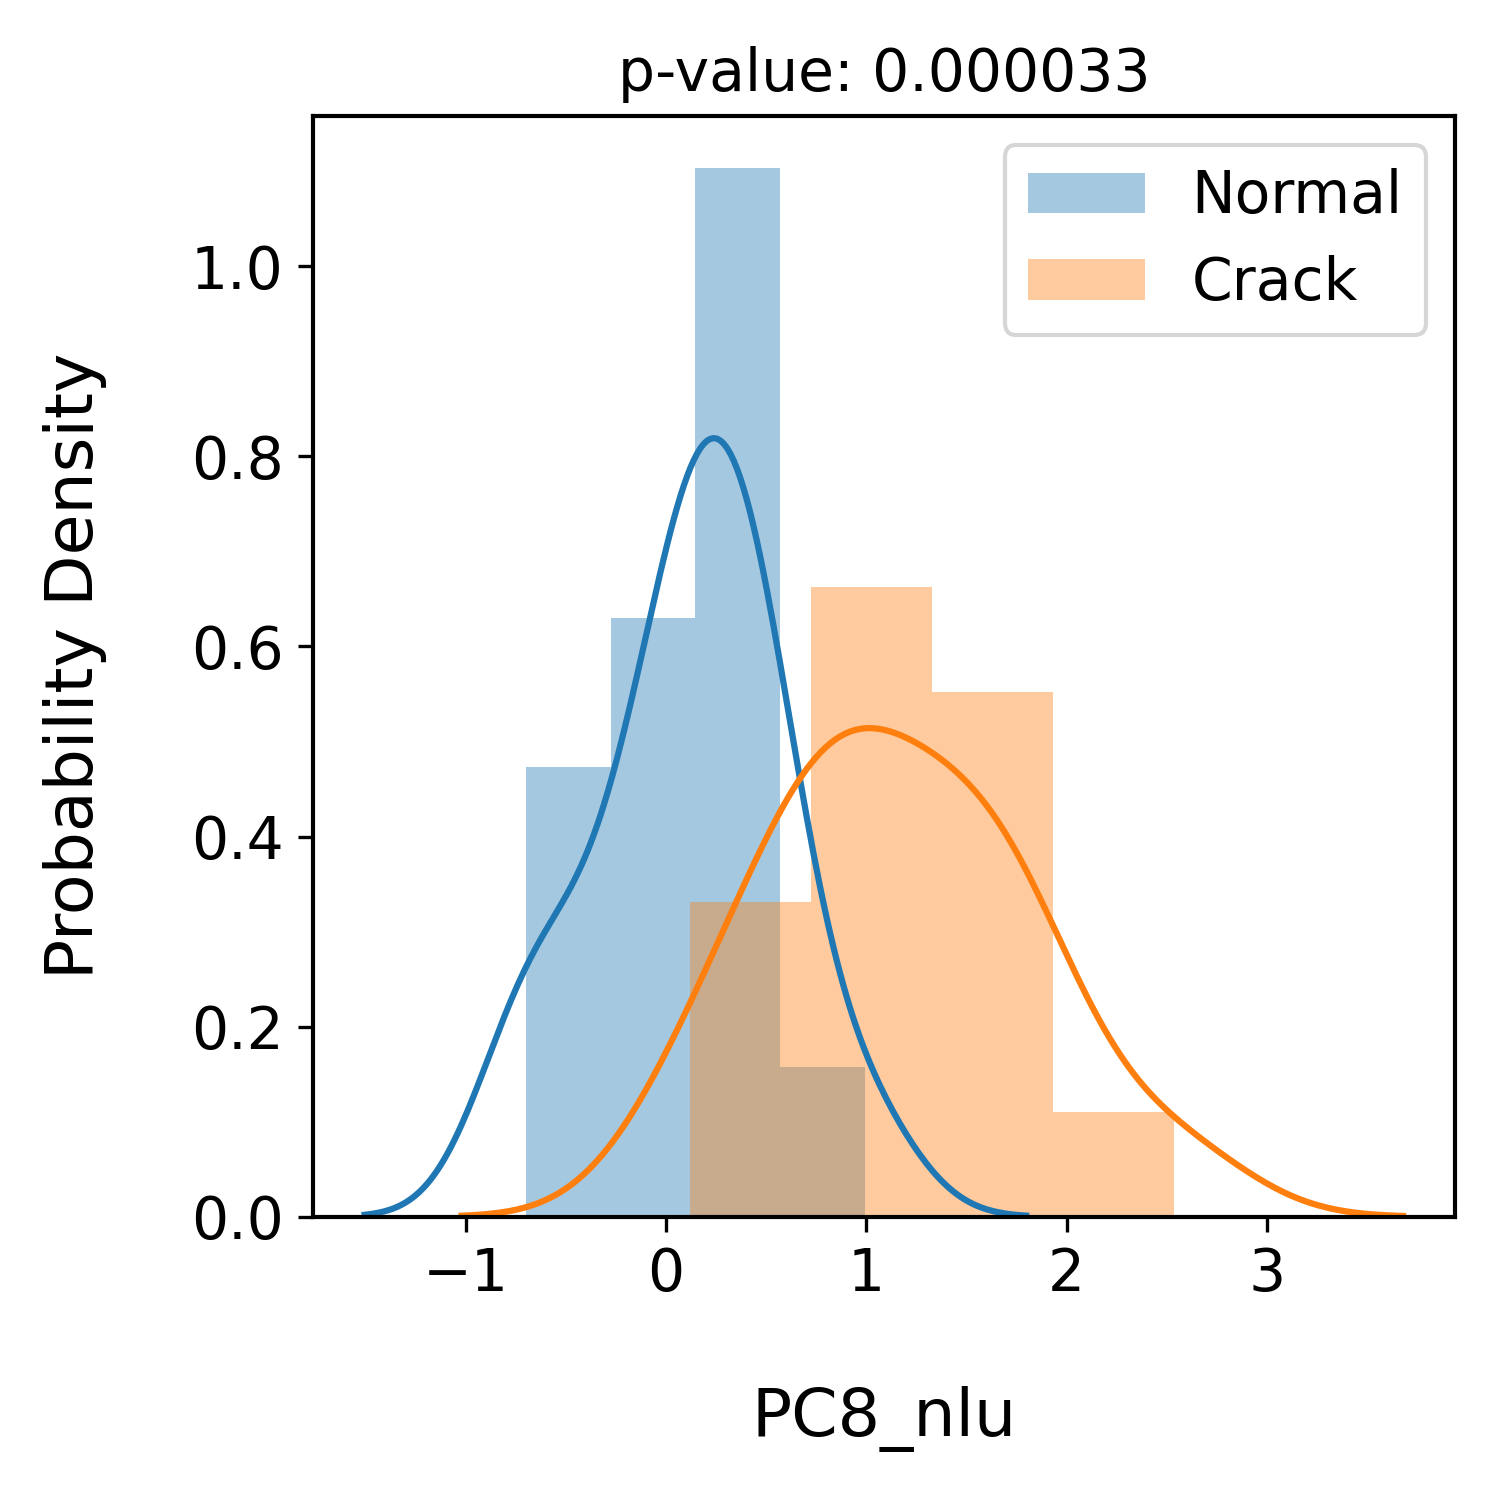
\includegraphics[width=0.8\textwidth]{fig/crack_detection_PC8_nlu.png}
    \caption{Principal component 8 of NLU signal}
  \end{subfigure}

  \caption{Probability density plots for selected LU and NLU features}
  \label{fig: crack detection feat dist}
\end{figure}